\chapter{Теорія ймовірності в контексті аналізу даних.}


\section{Основи теорії ймовірності.}

Теорія ймовірності це розділ математики, що вивчає закономірності випадкових явищ і дає змогу оцінити, наскільки ймовірною є та чи інша подія. 

Ніколи не можна точно знати, якою, наприклад, буде завтрашня погода. Проте маючи дані спостереження за регіоном на протязі певного періоду часу в даний сезон, можна оцінити, з якою ймовірністю завтра буде дощ. Спеціаліст з аналізу даних повинен вміти працювати з ймовірностями для того, щоб працювати з невизначеністю, прогнозувати майбутні події, оцінювати ризики та будувати моделі машинного навчання.

Теорія ймовірності лежить в основі багатьох алгоритмів машинного навчання, статистики, прогнозування часових рядів, аналізу ризиків і систем підтримки прийняття рішень.

Теорія ймовірності вивчає випадкові явища та закономірності їх виникнення. Центральними поняттями цієї теорії є випадковий експеримент, подія та ймовірність. Саме вони лежать в основі статистичного аналізу, машинного навчання, прогнозування, аналізу ризиків та багатьох інших методів інтелектуального аналізу даних.

\begin{lstlisting}
import random
import math
import numpy as np
from collections import Counter

pX = {1: 0.1, 2: 0.5, 3:0.4}
pWeather = {"sunny": 0.3, "rainy":0.2, "cloudy":0.4, "snowy":0.1}
print(pWeather["sunny"])
\end{lstlisting}

Результат:

\begin{console}
0.3
\end{console}

Випадковий експеримент — це дія або процес, результат якого наперед точно невідомий, хоча всі можливі результати можна перелічити. Прикладами випадкових експериментів є підкидання монети, кидання грального кубика, витягування карти з колоди, випадковий вибір клієнта із бази даних або визначення того, чи відкриє користувач рекламне повідомлення.

Елементарною подією називають окремий можливий результат випадкового експерименту. Наприклад, при киданні шестигранного кубика можливими елементарними подіями є випадіння чисел 1, 2, 3, 4, 5 або 6. Під час підкидання монети існує лише дві елементарні події: випадіння герба або цифри. 

Приклад: Кидання монети. Симулюємо 10 підкидувань, обчислюємо емпіричну ймовірність випадання «решки».

\begin{lstlisting}
tosses = [random.choice(["H", "T"]) for _ in range(10)]
print(tosses)

p_heads = tosses.count("H") / len(tosses)
print(f"P(Heads) approx. {p_heads:.2f}")
\end{lstlisting}

Результат:

\begin{console}
['H', 'T', 'T', 'H', 'H', 'H', 'H', 'T', 'T', 'T']
P(Heads) approx. 0.50
\end{console}

Множина всіх можливих елементарних подій називається простором елементарних подій, і позначається символом ($\Omega$).

Для кидання кубика $\Omega={1,2,3,4,5,6}$, для підкидання монети $\Omega={\text{герб},\ \text{цифра}}$. Будь-яка випадкова подія є підмножиною простору елементарних подій.

Ми називаємо дві події "незалежними", якщо однієї з них не впливає на ймовірність настання іншої. Наприклад, якщо двічі підкинути монету, результат другого підкидання не залежить від результату першого - якщо ми знаємо, що перший раз випала "решка", це нічого не каже нам про те, яким буде результат наступного підкидання. 

Для двох незалежних подій справедливою є наступна формула:

$$P(A\cap B)=P(A)\cdot P(B).$$

Наприклад, імовірність того, що при двох підкиданнях монети двічі випаде герб, дорівнює $\frac{1}{2}\cdot\frac{1}{2}=\frac{1}{4}$.



\subsection{Закон великих чисел.}

Одним із фундаментальних математичних законів теорії ймовірності є закон великих чисел.

Давайте подивимося, як емпірична ймовірність наближається до теоретичної ймовірності для різної кількості експериментів. Симулюємо підкидання монети 10, 100, 1000 та 10000 разів:

\begin{lstlisting}
def simulate_coin(n_tosses=1000):
    tosses = [random.choice(["H", "T"]) for _ in range(n_tosses)]
    return tosses.count("H") / n_tosses

for n in [10, 100, 1000, 10000]:
    print(f"{n} tosses -> P(Heads) approx. {simulate_coin(n):.3f}")
\end{lstlisting}

Результат:

\begin{console}
10 tosses -> P(Heads) approx. 0.200
100 tosses -> P(Heads) approx. 0.580
1000 tosses -> P(Heads) approx. 0.496
10000 tosses -> P(Heads) approx. 0.500
\end{console}

По мірі того, як число підкидувань зростає, ймовірність стабілізується около 0.5. Це є наглядним прикладом виконання закону великих чисел.

Закон великих чисел стверджує, що при багаторазовому повторенні однакового випадкового експерименту за однакових умов відносна частота появи певної події наближається до її теоретичної ймовірності. Для вищенаведеного прикладу із монетами, ця теоретична ймовірність рівна якраз 0.5.

Закон великих чисел пояснює, чому аналіз великих обсягів даних дозволяє отримувати більш надійні висновки.

Якщо вибірка містить дуже мало спостережень, випадкові коливання можуть суттєво спотворювати результати. Зі збільшенням кількості даних вплив випадковості зменшується, а оцінки характеристик генеральної сукупності стають точнішими. Саме тому в дослідженні даних використовуються якомога більші вибірки.

У машинному навчанні закон великих чисел є однією з причин, чому якість моделей зазвичай покращується зі збільшенням обсягу навчальних даних.


\section{Використання NumPy для роботи з розподілами ймовірностей.}

\subsection{Рівномірний розподіл.}

В наступному прикладі генеруємо випадкові числа між 0 та 1, та виводимо ймовірність того, що значення із цього розподілу менше за 0.5.

\begin{lstlisting}
import numpy as np

samples = np.random.rand(5)
print(samples)

p = np.mean(samples < 0.5)
print("P(X < 0.5) approx.", p)
\end{lstlisting}

Результат:

\begin{console}
[0.75955599 0.02132349 0.45415367 0.32714836 0.93499247]
P(X < 0.5) approx. 0.6
\end{console}


\subsection{Гаусівський розподіл.}

Гаусівський розподіл (Normal, Gaussian Distribution) є розподілом по дійсних числах і, ймовірно, є найпоширенішим розподілом у науці про дані (я не кажу, що це найпоширеніший розподіл у самих даних, а в науці про дані як галузі). Це пояснюється багатьма приємними властивостями розподілу: він легко інтегрується, має природний багатовимірний аналог, а також тим фактом, про який ми поговоримо в декількох лекціях, що певні розподіли даних середніх значень вибірки мають тенденцію до гаусівського розподілу (так звана центральна гранична теорема). Гаусівський розподіл має "дзвоноподібну" функцію щільності, яка, ймовірно, знайома багатьом людям.

Згенеруємо гаусівський розподіл із середнім 0 та відхиленням 1 засобами NumPy:

\begin{lstlisting}
samples = np.random.normal(loc=0, scale=1, size=10000)
print("Mean:", np.mean(samples))
print("Std Dev:", np.std(samples))

import matplotlib.pyplot as plt

plt.hist(samples, bins=30, density=True, alpha=0.6)
plt.title("Normal Distribution (nu=0, sigma=1)")
plt.xlabel("x")
plt.ylabel("Density")
plt.show()
\end{lstlisting}

Результат:

\begin{console}
Mean: -0.002846126267790618
Std Dev: 0.9992466721005764
\end{console}

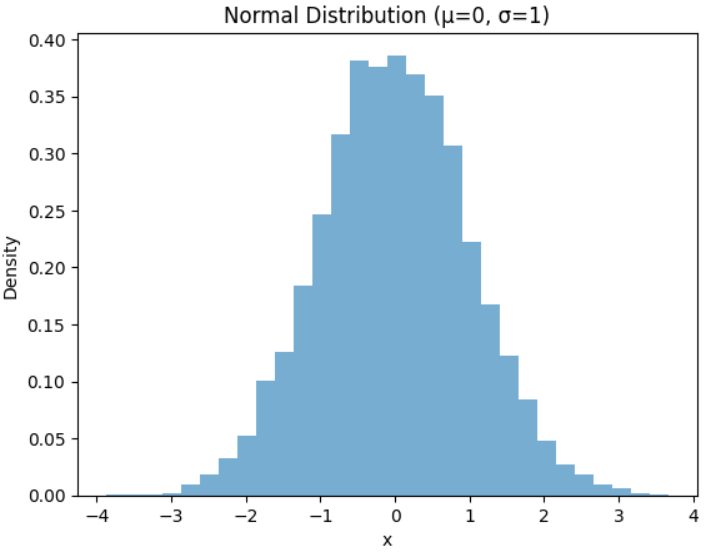
\includegraphics[scale=0.75]{img/107-1}

Можна навести багато прикладів, де зустрічається нормальний розподіл: зріст людей (запишіть ріст ваших одногруників - ви побачите, що він підпадає саме під нормальний розподіл), результати іспитів, середній час виконання тієї чи іншої дії. Багато математичних моделей було розроблено із припущенням, що дані мають саме нормальний розподіл. 



\subsection{Дискретні розподіли.}

Задамо параметри розподілу: кількість випробувань 10 та ймовірність успіху 0.5. Обчислимо ймовірність випадання рівно 3 "решок" за 10 підкидань, та кумулятивну ймовірність $P(X \leq 3)$.

\begin{lstlisting}
from scipy.stats import binom

n = 10   
p = 0.5  

prob = binom.pmf(k=3, n=n, p=p)
print(f"P(X=3) = {prob:.4f}")

cum_prob = binom.cdf(k=3, n=n, p=p)
print(f"P(X <= 3) = {cum_prob:.4f}")

x = np.arange(0, 11)
y = binom.pmf(x, n, p)

plt.bar(x, y)
plt.xlabel("Number of Heads")
plt.ylabel("Probability")
plt.title("Binomial(n=10, p=0.5)")
plt.show()
\end{lstlisting}

Результат:

\begin{console}
P(X=3) = 0.1172
P(X <= 3) = 0.1719
\end{console}

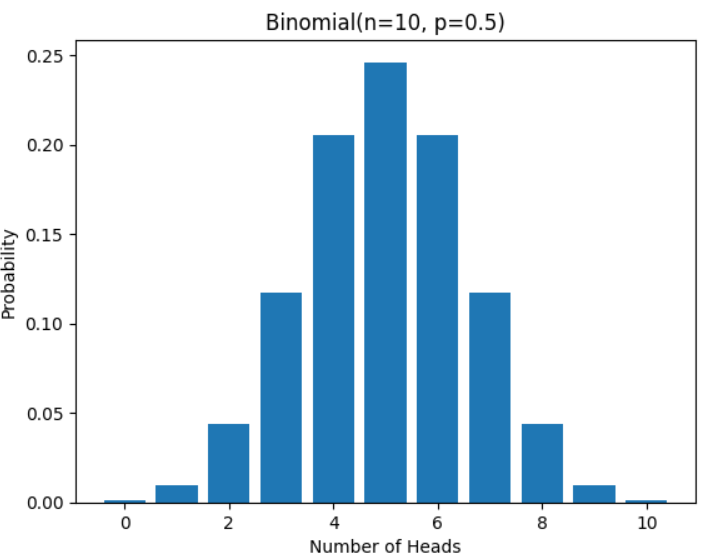
\includegraphics[scale=0.75]{img/107-2}



\section{Теорема Байєса.}

Обчислимо ймовірність захворювання за умови позитивного результату тесту. Якщо 1 $\%$ населення хворіє, то P(Захворювання) = 0,01. Точність тесту становить 99 $\%$, то  P(Позитивний результат | Захворювання) = 0,99;  P(Позитивний результат | Відсутність захворювання) = 0,01. Обчислимо P(Захворювання | Позитивний результат):

\begin{lstlisting}
P_D = 0.01
P_Pos_given_D = 0.99
P_Pos_given_notD = 0.01

P_Pos = P_Pos_given_D * P_D + P_Pos_given_notD * (1 - P_D)

P_D_given_Pos = (P_Pos_given_D * P_D) / P_Pos
print(f"P(Disease | Positive Test) = {P_D_given_Pos:.3f}")
\end{lstlisting}

Результат:

\begin{console}
P(Disease | Positive Test) = 0.500
\end{console}


\ding{46} \textbf{Питання для самоконтролю.}

\begin{enumerate}
\item Що вивчає теорія ймовірності?
\item Чому теорія ймовірності є важливою для інтелектуального аналізу даних?
\item Що таке випадковий експеримент?
\item Що таке елементарна подія?
\item Що називають простором елементарних подій?
\item Що таке випадкова подія?
\item Які види подій розрізняють у теорії ймовірності?
\item Що таке достовірна подія?
\item Що таке неможлива подія?
\item Які події називають несумісними?
\item Які події називають незалежними?
\item Як визначається ймовірність події?
\item Які властивості має ймовірність?
\item Як обчислюється ймовірність суми несумісних подій?
\item Як обчислюється ймовірність суми довільних подій?
\item Як обчислюється ймовірність перетину незалежних подій?
\item Що таке умовна ймовірність?
\item Як обчислюється умовна ймовірність?
\item У чому полягає правило множення ймовірностей?
\item Що таке повна група подій?
\item У чому полягає формула повної ймовірності?
\item Що таке випадкова величина?
\item Чим дискретна випадкова величина відрізняється від неперервної?
\item Що таке закон розподілу випадкової величини?
\item Що таке функція розподілу?
\item Що таке математичне сподівання?
\item Як обчислюється математичне сподівання дискретної випадкової величини?
\item Який практичний зміст має математичне сподівання?
\item Що таке дисперсія випадкової величини?
\item Для чого використовується стандартне відхилення?
\item Що показує дисперсія в аналізі даних?
\item У чому полягає закон великих чисел?
\item Яке практичне значення закону великих чисел?
\item Як закон великих чисел застосовується в машинному навчанні?
\item Що таке біноміальний розподіл?
\item У яких задачах застосовується біноміальний розподіл?
\item Що таке розподіл Бернуллі?
\item Чим розподіл Бернуллі відрізняється від біноміального?
\item Що таке нормальний розподіл?
\item Якими властивостями характеризується нормальний розподіл?
\item Чому нормальний розподіл часто зустрічається в реальних даних?
\item Що таке розподіл Пуассона?
\item У яких практичних задачах застосовується розподіл Пуассона?
\item У чому полягає теорема Байеса?
\item Як обчислюється апостеріорна ймовірність за теоремою Байеса?
\item Яке практичне значення має теорема Байеса для аналізу даних?
\item Як теорема Байеса використовується в задачах класифікації?
\item Що таке наївний байєсівський класифікатор і на якому припущенні він ґрунтується?
\item Яку роль відіграють ймовірнісні моделі в сучасному інтелектуальному аналізі даних?
\item Чому розуміння основ теорії ймовірності є необхідним для побудови моделей машинного навчання та прийняття рішень на основі даних?
\end{enumerate}
